%% BioMed_Central_Tex_Template_v1.05
%%                                      %
%  bmc_article.tex            ver: 1.05 %
%                                       %


%%%%%%%%%%%%%%%%%%%%%%%%%%%%%%%%%%%%%%%%%
%%                                     %%
%%  LaTeX template for BioMed Central  %%
%%     journal article submissions     %%
%%                                     %%
%%         <27 January 2006>           %%
%%                                     %%
%%                                     %%
%% Uses:                               %%
%% cite.sty, url.sty, bmc_article.cls  %%
%% ifthen.sty. multicol.sty		       %%
%%									   %%
%%                                     %%
%%%%%%%%%%%%%%%%%%%%%%%%%%%%%%%%%%%%%%%%%


%%%%%%%%%%%%%%%%%%%%%%%%%%%%%%%%%%%%%%%%%%%%%%%%%%%%%%%%%%%%%%%%%%%%%
%%                                                                 %%	
%% For instructions on how to fill out this Tex template           %%
%% document please refer to Readme.pdf and the instructions for    %%
%% authors page on the biomed central website                      %%
%% http://www.biomedcentral.com/info/authors/                      %%
%%                                                                 %%
%% Please do not use \input{...} to include other tex files.       %%
%% Submit your LaTeX manuscript as one .tex document.              %%
%%                                                                 %%
%% All additional figures and files should be attached             %%
%% separately and not embedded in the \TeX\ document itself.       %%
%%                                                                 %%
%% BioMed Central currently use the MikTex distribution of         %%
%% TeX for Windows) of TeX and LaTeX.  This is available from      %%
%% http://www.miktex.org                                           %%
%%                                                                 %%
%%%%%%%%%%%%%%%%%%%%%%%%%%%%%%%%%%%%%%%%%%%%%%%%%%%%%%%%%%%%%%%%%%%%%


\NeedsTeXFormat{LaTeX2e}[1995/12/01]
\documentclass[10pt]{bmc_article}    



% Load packages
\usepackage{cite} % Make references as [1-4], not [1,2,3,4]
\usepackage{url}  % Formatting web addresses  
\usepackage{ifthen}  % Conditional 
\usepackage{multicol}   %Columns
\usepackage[utf8]{inputenc} %unicode support
%\usepackage[applemac]{inputenc} %applemac support if unicode package fails
%\usepackage[latin1]{inputenc} %UNIX support if unicode package fails
\urlstyle{rm}
 
 
%%%%%%%%%%%%%%%%%%%%%%%%%%%%%%%%%%%%%%%%%%%%%%%%%	
%%                                             %%
%%  If you wish to display your graphics for   %%
%%  your own use using includegraphic or       %%
%%  includegraphics, then comment out the      %%
%%  following two lines of code.               %%   
%%  NB: These line *must* be included when     %%
%%  submitting to BMC.                         %% 
%%  All figure files must be submitted as      %%
%%  separate graphics through the BMC          %%
%%  submission process, not included in the    %% 
%%  submitted article.                         %% 
%%                                             %%
%%%%%%%%%%%%%%%%%%%%%%%%%%%%%%%%%%%%%%%%%%%%%%%%%                     


%\def\includegraphic{}
%\def\includegraphics{}
\usepackage{graphicx}



\setlength{\topmargin}{0.0cm}
\setlength{\textheight}{21.5cm}
\setlength{\oddsidemargin}{0cm} 
\setlength{\textwidth}{16.5cm}
\setlength{\columnsep}{0.6cm}

\newboolean{publ}

%%%%%%%%%%%%%%%%%%%%%%%%%%%%%%%%%%%%%%%%%%%%%%%%%%
%%                                              %%
%% You may change the following style settings  %%
%% Should you wish to format your article       %%
%% in a publication style for printing out and  %%
%% sharing with colleagues, but ensure that     %%
%% before submitting to BMC that the style is   %%
%% returned to the Review style setting.        %%
%%                                              %%
%%%%%%%%%%%%%%%%%%%%%%%%%%%%%%%%%%%%%%%%%%%%%%%%%%
 

%Review style settings
%\newenvironment{bmcformat}{\begin{raggedright}\baselineskip20pt\sloppy\setboolean{publ}{false}}{\end{raggedright}\baselineskip20pt\sloppy}

%Publication style settings
\newenvironment{bmcformat}{\fussy\setboolean{publ}{true}}{\fussy}



% Begin ...
\begin{document}
\begin{bmcformat}


%%%%%%%%%%%%%%%%%%%%%%%%%%%%%%%%%%%%%%%%%%%%%%
%%                                          %%
%% Enter the title of your article here     %%
%%                                          %%
%%%%%%%%%%%%%%%%%%%%%%%%%%%%%%%%%%%%%%%%%%%%%%

\title{Applications of InChI in cheminformatics with CDK and Bioclipse}
 
%%%%%%%%%%%%%%%%%%%%%%%%%%%%%%%%%%%%%%%%%%%%%%
%%                                          %%
%% Enter the authors here                   %%
%%                                          %%
%% Ensure \and is entered between all but   %%
%% the last two authors. This will be       %%
%% replaced by a comma in the final article %%
%%                                          %%
%% Ensure there are no trailing spaces at   %% 
%% the ends of the lines                    %%     	
%%                                          %%
%%%%%%%%%%%%%%%%%%%%%%%%%%%%%%%%%%%%%%%%%%%%%%



\author{Ola Spjuth\correspondingauthor$^{1}$%
         \email{OS\correspondingauthor : ola.spjuth@farmbio.uu.se}%
      \and
         Arvid Berg$^1$%
         \email{AB: arvid.berg@farmbio.uu.se}%
      \and
         Samuel Adams$^2$%
         \email{SA: sea36@cam.ac.uk}%
      \and    
         Egon Willighagen$^3$%
         \email{EW: egon.willighagen@maastrichtuniversity.nl}%
      }
      
      

%%%%%%%%%%%%%%%%%%%%%%%%%%%%%%%%%%%%%%%%%%%%%%
%%                                          %%
%% Enter the authors' addresses here        %%
%%                                          %%
%%%%%%%%%%%%%%%%%%%%%%%%%%%%%%%%%%%%%%%%%%%%%%

\address{\\
\iid(1) Department of Pharmaceutical Biosciences, Uppsala University, 751 24 Uppsala, Sweden\\
\iid(2) Unilever Centre for Molecular Sciences Informatics, University Chemical Laboratory, Cambridge, CB2 1EW, United Kingdom\\
\iid(3) Maastricht uni...}

%}



\maketitle

%%%%%%%%%%%%%%%%%%%%%%%%%%%%%%%%%%%%%%%%%%%%%%
%%                                          %%
%% The Abstract begins here                 %%
%%                                          %%
%% The Section headings here are those for  %%
%% a Research article submitted to a        %%
%% BMC-Series journal.                      %%  
%%                                          %%
%% If your article is not of this type,     %%
%% then refer to the Instructions for       %%
%% authors on http://www.biomedcentral.com  %%
%% and change the section headings          %%
%% accordingly.                             %%   
%%                                          %%
%%%%%%%%%%%%%%%%%%%%%%%%%%%%%%%%%%%%%%%%%%%%%%


\begin{abstract}
        % Do not use inserted blank lines (ie \\) until main body of text.

%        \paragraph*{Background:} Text for this section of the abstract. 
      
%        \paragraph*{Results:} Text for this section of the abstract \ldots

%        \paragraph*{Conclusions:} Text for this section of the abstract \ldots
        
We describe the integration of InChI into the Bioclipse workbench using the Chemistry Development Kit (CDK) cheminformatics library. The CDK project packages the InChI binaries in a module and offers easy access from Java using the CDK API, which internally uses the JNI-InChI bridge to InChI from Java. Bioclipse packages and offers InChI as a dynamic OSGi bundle that can easily be used by any OSGi-compliant software. InChI is a key component in Bioclipse and is calculated on the fly and displayed when visualizing and editing chemical structures in 2D. We demonstrate the utility of InChI with various applications in CDK and Bioclipse, such as decision support for chemical liability assessment, tautomer generation, and for knowledge aggregation using a linked data approach.        
        
        
\end{abstract}



\ifthenelse{\boolean{publ}}{\begin{multicols}{2}}{}




%%%%%%%%%%%%%%%%%%%%%%%%%%%%%%%%%%%%%%%%%%%%%%
%%                                          %%
%% The Main Body begins here                %%
%%                                          %%
%% The Section headings here are those for  %%
%% a Research article submitted to a        %%
%% BMC-Series journal.                      %%  
%%                                          %%
%% If your article is not of this type,     %%
%% then refer to the instructions for       %%
%% authors on:                              %%
%% http://www.biomedcentral.com/info/authors%%
%% and change the section headings          %%
%% accordingly.                             %% 
%%                                          %%
%% See the Results and Discussion section   %%
%% for details on how to create sub-sections%%
%%                                          %%
%% use \cite{...} to cite references        %%
%%  \cite{koon} and                         %%
%%  \cite{oreg,khar,zvai,xjon,schn,pond}    %%
%%  \nocite{smith,marg,hunn,advi,koha,mouse}%%
%%                                          %%
%%%%%%%%%%%%%%%%%%%%%%%%%%%%%%%%%%%%%%%%%%%%%%




%%%%%%%%%%%%%%%%
%% Background %%
%%
\section*{Background}

It is of great importance that chemical structures can be serialized in standard formats in order to enable exchange and linking of chemical information. The IUPAC Chemical Identifier (InChI)~\cite{Stein2003} is such a standardized identifier for chemical structures, which lately has seen a great adoption in the cheminformatics community~\cite{OBoyle:2011fk}. Two important use cases are querying for exact matches in databases, and linking chemical structures using semantic web technologies. The official implementation of InChI is in C as a library, in order to provide a single implementation that everyone can use. This however limits its use in other programming languages such as Java. We here describe the packaging of InChI in Java, to enable frameworks and applications written in this language to take advantage of the benefits of InChI. We present the integration of InChI in the cheminformatics library the Chemistry Development Kit as well as the graphical workbench Bioclipse. We also provide demonstrations where InChI is used in decision support for chemical liability assessment, for tautomer generation, and for knowledge aggregation using a linked data approach.
 




%%%%%%%%%%%%%%%%%%%%%%%%%%%%
%% Results and Discussion %%
%%
\section*{Results and Discussion}

\subsection*{Packaging InChI in a Java library [EGON, SAM]}
JNI-InChI is the packaging of the InChI libraries in portable Java libraries using the Java Native Interface. Available on Sourceforge under Gnu Lesser General Public License (LGPL)\dots TBC

%BELOW IS FROM BO5yearsOnPaper

%The Blue Obelisk project JNI-InChI~\cite{jni-inchi} was established in 2006 to solve this problem by using the Java Native Interface framework to provide transparent access to the InChI library from within Java and other Java Virtual Machine (JVM) based languages, supporting the wider adoption of this standard identifier by the chemistry community.

%The Java Native Interface framework provides a mechanism for code running inside the JVM, to place calls to libraries written in languages such as C, C++ and Fortran, and compiled into native, machine specific, code. JNI-InChI provides a thin C wrapper, with corresponding Java code, around the IUPAC InChI library, exposing the InChI library's functionality to the JVM. To overcome the need to have the correct InChI library pre-installed on a system, JNI-InChI comes with a variety of precompiled native binaries and automatically extracts and deploys the correct one for the detected operating system and architecture. The JNI-InChI library comes with native binaries supporting a range of operating systems and architectures; the current version has binaries for 32- and 64-bit Windows, Linux and Solaris, 64-bit FreeBSD and 64-bit Intel-based Mac OS X - a number of which are not supported by the original IUPAC distribution of InChI. The JNI-InChI project has matured to support the full range of functionality of the InChI C library: structure-to-InChI, InChI-to-structure, AuxInfo-to-structure, InChIKey generation, and InChI and InChIKey validation. JNI-InChI provides the InChI functionality for a number of Open Source projects, including the Chemistry Development Kit, Bioclipse and CMLXOM/JUMBO, and is also used by commercial applications and internally in a number of companies. Through its widespread use and Open Source development model, a number of issues in earlier versions of the software have been identified and resolved, and JNI-InChI now offers a robust tool for working with InChIs in the JVM.





\subsection*{Integration of InChI in CDK [EGON]}
TBC


\begin{figure*}[!hb]
\begin{center}
	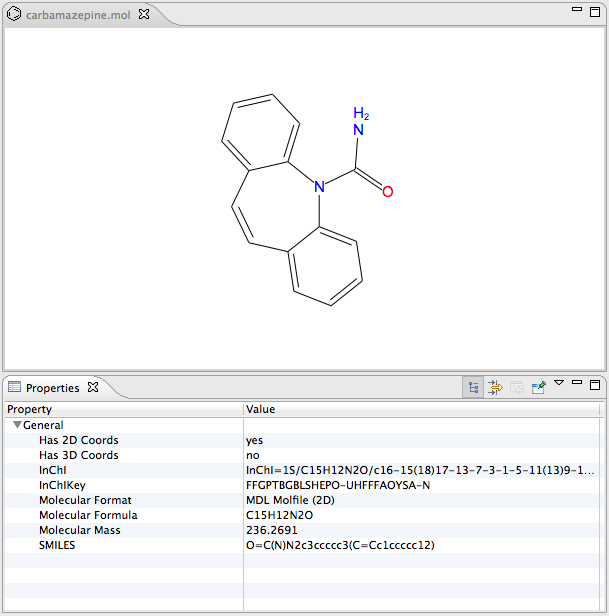
\includegraphics[width=9cm]{carbamazepine-props.png}

\caption{Part of the Bioclipse workbench showing the chemical structure for the drug carbamazepine, with the InChI and InChIKey displayed as properties in the bottom canvas. Editing the chemical structure instantly triggers a recalculation of these properties.}
\label{fig:carba-prop}
\end{center}
\end{figure*}


\subsection*{Provisioning of InChI as OSGi bundles [OLA, ARVID]}
OSGi~\cite{osgi} is a standard for dynamic module system in Java, allowing for easy provisioning and interoperability of modules, mainly containing compiled Java code but also associated data. The Bioclipse projects has developed OSGi bundles for InChI by wrapping the JNI-InChI libraries, which required some modifications... class loaders... The OSGi bundles are available from a p2 repository (TBC), as well as downloadable from the web page (TBC)\dots Having OSGi bundles with InChI enables easy access from all plugins supporting this module technology, which in 

Cheminformatics tools that makes use of the OSGi module system includes Knime~\cite{Warr:2012kx}, Cytoscape~\cite{Shannon:2003zr}, Taverna~\cite{Oinn:2004ys,Truszkowski:2011vn}, and Bioclipse~\cite{Spjuth:2007ve}.

\subsection*{Integration of InChI in Bioclipse  [OLA]}
Bioclipse is a workbench for the life sciences where cheminformatics is the most developed functionality. Key features of Bioclipse includes import, export and editing of chemical structures in various file formats, as well as visualizations and various property calculations - all features available from both a graphical workbench as well as a built-in scripting language (Bioclipse Scripting Language, or BSL)~\cite{Spjuth:2009ly}. As a Rich Client built on the Eclipse Rich Client Platform (RCP), Bioclipse inherits an extensible architecture implementing the OSGi standard. By adding the previously described InChI OSGi bundles to Bioclipse, Bioclipse exposes InChI calculation as a key feature in the workbench, and InChI is calculated on all structure modifications and visualized as a general property in the workbench window (see Figure~\ref{fig:carba-prop}). Bioclipse supports both the generation of standard and non-standard InChIs, and a preference allows for selecting between the different versions.

\begin{figure*}[!hb]
\begin{center}
	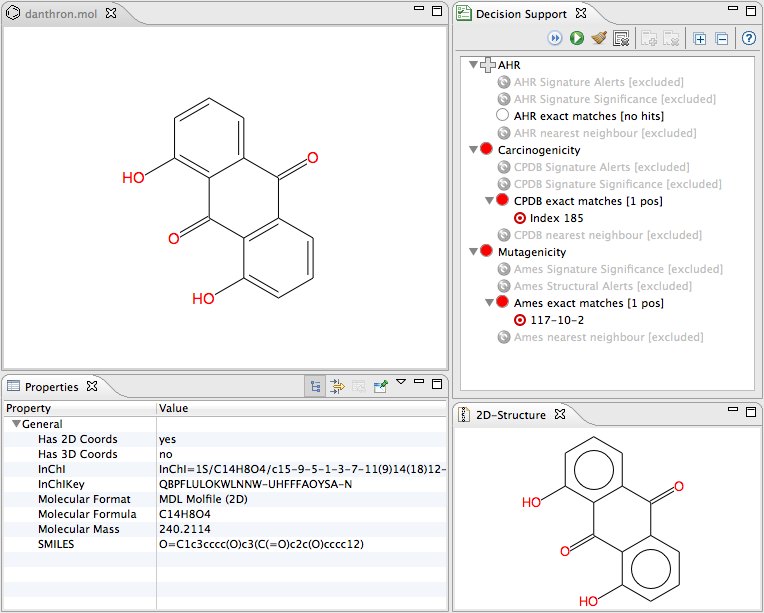
\includegraphics[width=9cm]{danthron-ds.png}

\caption{Part of the Bioclipse workbench showing the Decision Support feature with three exact matches enabled (right canvas) and the chemical structure of the withdrawn drug Danthron. We see that the data sets for CPDB~\cite{Fitzpatrick:2008dp} and Ames Mutagenicity~\cite{Kazius:2005pv} both gives an exact match, and that this compound has previously been shown to be positive (mutagen) in an Ames Mutagenicity test as well as positive for an in vivo carcinogenicity test included in the Carcinogenicity Potency Database.}
\label{fig:danth-ds}
\end{center}
\end{figure*}




	

\begin{verbatim}
  mol=cdk.fromSMILES("OC=O")
  sinchi = inchi.generate(mol);
  inchi = inchi.generate(mol), "FixedH");
\end{verbatim}


%%%%%%%%%%
%APPLICATIONS
%%%%%%%%%%
\subsection*{Applications of InChI in cheminformatics}



\subsubsection*{Decision support in computational pharmacology [OLA]}
In chemical safety assessment, the first step when faced with a new chemical structure is to see weather it already has been synthesized, and if any in vitro assays or in vivo studies have been performed. Given the large size of knowledge bases in companies and organizations, exact database lookups have become ubiquitous tools and used on a daily basis. Bioclipse Decision Support provides a framework for running exact match queries against a library of chemical structures, which was demonstrated for 3 open safety endpoints~\cite{Spjuth:2011qf}. An example query can be seen in Figure~\ref{fig:danth-ds}.


\subsubsection*{b) Linked data in Bioclipse and CDK using InChI (e.g. Isbjorn) [EGON]}
TBC

\subsubsection*{c) CDK tautomer calculation in Bioclipse moltable [EGON]}


{\footnotesize 
\begin{verbatim}

// no aromatic rings that make it hard to see where the
// double bonds are
jcpglobal.setShowAromaticity(false);

inputSMILES = "c1ccccc1O";
inputName = "phenol";
inchi.generate(cdk.fromSMILES(inputSMILES))
tautomers = cdk.getTautomers(
  cdk.fromSMILES(inputSMILES)
)

file = "/Virtual/" + inputName + ".sdf";
cdk.saveSDFile(file, tautomers);
ui.open(file);

\end{verbatim}
}


%%%%%%%%%%%%%%%%%%%%%%
\section*{Conclusions}
Summarize what we have done and the implications.\\
Talk about problems with InChI versions. We overcome some with prefs page allowing users to select InChI version.


  
%%%%%%%%%%%%%%%%%%
%\section*{Methods}
%  \subsection*{Methods sub-heading for this section}
%    Text for this sub-section \ldots


    
%%%%%%%%%%%%%%%%%%%%%%%%%%%%%%%%
\section*{Authors contributions}
    Text for this section \ldots

    

%%%%%%%%%%%%%%%%%%%%%%%%%%%
\section*{Acknowledgements}
  \ifthenelse{\boolean{publ}}{\small}{}
  Text for this section \ldots


 
%%%%%%%%%%%%%%%%%%%%%%%%%%%%%%%%%%%%%%%%%%%%%%%%%%%%%%%%%%%%%
%%                  The Bibliography                       %%
%%                                                         %%              
%%  Bmc_article.bst  will be used to                       %%
%%  create a .BBL file for submission, which includes      %%
%%  XML structured for BMC.                                %%
%%                                                         %%
%%                                                         %%
%%  Note that the displayed Bibliography will not          %% 
%%  necessarily be rendered by Latex exactly as specified  %%
%%  in the online Instructions for Authors.                %% 
%%                                                         %%
%%%%%%%%%%%%%%%%%%%%%%%%%%%%%%%%%%%%%%%%%%%%%%%%%%%%%%%%%%%%%


{\ifthenelse{\boolean{publ}}{\footnotesize}{\small}
 \bibliographystyle{bmc_article}  % Style BST file
  \bibliography{inchi-cdk-bioclipse} }     % Bibliography file (usually '*.bib' ) 

%%%%%%%%%%%

\ifthenelse{\boolean{publ}}{\end{multicols}}{}

%%%%%%%%%%%%%%%%%%%%%%%%%%%%%%%%%%%
%%                               %%
%% Figures                       %%
%%                               %%
%% NB: this is for captions and  %%
%% Titles. All graphics must be  %%
%% submitted separately and NOT  %%
%% included in the Tex document  %%
%%                               %%
%%%%%%%%%%%%%%%%%%%%%%%%%%%%%%%%%%%

%%
%% Do not use \listoffigures as most will included as separate files

%\section*{Figures}
%  \subsection*{Figure 1 - Sample figure title}
%      A short description of the figure content
%      should go here.
%
%  \subsection*{Figure 2 - Sample figure title}
%      Figure legend text.



%%%%%%%%%%%%%%%%%%%%%%%%%%%%%%%%%%%
%%                               %%
%% Tables                        %%
%%                               %%
%%%%%%%%%%%%%%%%%%%%%%%%%%%%%%%%%%%

%% Use of \listoftables is discouraged.
%%
%\section*{Tables}
%  \subsection*{Table 1 - Sample table title}
%    Here is an example of a \emph{small} table in \LaTeX\ using  
%    \verb|\tabular{...}|. This is where the description of the table 
%    should go. \par \mbox{}
%    \par
%    \mbox{
%      \begin{tabular}{|c|c|c|}
%        \hline \multicolumn{3}{|c|}{My Table}\\ \hline
%        A1 & B2  & C3 \\ \hline
%        A2 & ... & .. \\ \hline
%        A3 & ..  & .  \\ \hline
%      \end{tabular}
%      }
%  \subsection*{Table 2 - Sample table title}
%    Large tables are attached as separate files but should
%    still be described here.



%%%%%%%%%%%%%%%%%%%%%%%%%%%%%%%%%%%
%%                               %%
%% Additional Files              %%
%%                               %%
%%%%%%%%%%%%%%%%%%%%%%%%%%%%%%%%%%%

%\section*{Additional Files}
%  \subsection*{Additional file 1 --- Sample additional file title}
%    Additional file descriptions text (including details of how to
%    view the file, if it is in a non-standard format or the file extension).  This might
%    refer to a multi-page table or a figure.
%
%  \subsection*{Additional file 2 --- Sample additional file title}
%    Additional file descriptions text.


\end{bmcformat}
\end{document}







